\begin{frame}{Why Recover 3D from Images}
  \begin{columns}[T,onlytextwidth]
    \column{0.46\textwidth}
      \begin{itemize}\footnotesize\itemsep0.35em
        \item A camera maps the 3D world onto a 2D image and discards depth: every point on a ray through the camera centre lands on the same pixel.
        \item Size and distance trade off. An object twice as tall and twice as far away covers the same pixels, so one image cannot separate a small near object from a large far one.
        \item Many tasks need metric 3D, in metres: robot navigation and grasping, autonomous driving (the distance to the car ahead), augmented reality (AR) content that stays anchored to real surfaces, and mapping or inspection of buildings and sites.
        \item Getting depth back needs extra information: a second view, camera motion, an object of known size, or priors learned from data.
      \end{itemize}
    \column{0.52\textwidth}
      \centering
      \vspace{0.4em}
      \begin{tikzpicture}[font=\sffamily\scriptsize, >=latex, scale=0.97, every node/.style={transform shape}]
        \draw[dashed, gray] (0,0) -- (6.1,0) node[right, black] {$Z$};
        \draw[thick, blue!60!black] (1,-0.35) -- (1,1.05) node[above] {image plane};
        \draw[thick, red!70!black, ->] (0,0) -- (6.1,2.44);
        \draw[line width=2.4pt, green!45!black] (1.8,0) -- (1.8,0.72);
        \draw[line width=2.4pt, green!45!black] (5.4,0) -- (5.4,2.16);
        \draw[line width=2.4pt, green!45!black] (1,0) -- (1,0.4);
        \fill (0,0) circle (1.6pt) node[below=2pt] {camera centre};
        \fill[red!70!black] (1,0.4) circle (1.6pt) node[above left=1pt and 0pt, black] {pixel};
        \fill[red!70!black] (1.8,0.72) circle (1.6pt) node[above left=1pt and -2pt, black] {$\mathbf{X}_1$};
        \fill[red!70!black] (3.6,1.44) circle (1.6pt) node[above left=1pt and -2pt, black] {$\mathbf{X}_2$};
        \fill[red!70!black] (5.4,2.16) circle (1.6pt) node[above left=1pt and -2pt, black] {$\mathbf{X}_3$};
        \node[below] at (1.8,0) {near, small};
        \node[below] at (5.4,0) {far, large};
      \end{tikzpicture}\\[0.5em]
      {\scriptsize $\mathbf{X}_1$, $\mathbf{X}_2$ and $\mathbf{X}_3$ lie on one ray and image to the same pixel. The far object (green) is three times taller and three times farther away than the near one, so their images coincide.\par}
  \end{columns}
\end{frame}

\begin{frame}{Four Problems, One Geometry}
  \centering
  \resizebox{\textwidth}{!}{%
  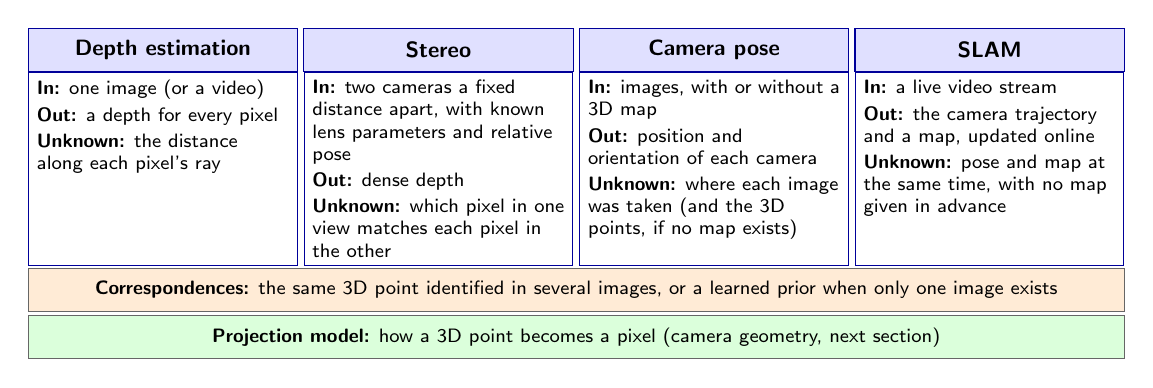
\begin{tikzpicture}[font=\sffamily\scriptsize, >=latex,
      head/.style={draw=blue!60!black, fill=blue!12, minimum width=3.42cm, minimum height=0.55cm, font=\sffamily\footnotesize\bfseries},
      body/.style={draw=blue!60!black, fill=white, anchor=north, inner sep=3pt},
      slab/.style={draw=black!60, minimum width=13.92cm, minimum height=0.55cm, align=center}]
    \node[head] at (1.75,3.3) {Depth estimation};
    \node[body] at (1.75,3.025) {\parbox[t][2.25cm][t]{3.2cm}{\raggedright\hyphenpenalty10000 \textbf{In:} one image (or a video)\\[0.2em] \textbf{Out:} a depth for every pixel\\[0.2em] \textbf{Unknown:} the distance along each pixel's ray}};
    \node[head] at (5.25,3.3) {Stereo};
    \node[body] at (5.25,3.025) {\parbox[t][2.25cm][t]{3.2cm}{\raggedright\hyphenpenalty10000 \textbf{In:} two cameras a fixed distance apart, with known lens parameters and relative pose\\[0.2em] \textbf{Out:} dense depth\\[0.2em] \textbf{Unknown:} which pixel in one view matches each pixel in the other}};
    \node[head] at (8.75,3.3) {Camera pose};
    \node[body] at (8.75,3.025) {\parbox[t][2.25cm][t]{3.2cm}{\raggedright\hyphenpenalty10000 \textbf{In:} images, with or without a 3D map\\[0.2em] \textbf{Out:} position and orientation of each camera\\[0.2em] \textbf{Unknown:} where each image was taken (and the 3D points, if no map exists)}};
    \node[head] at (12.25,3.3) {SLAM};
    \node[body] at (12.25,3.025) {\parbox[t][2.25cm][t]{3.2cm}{\raggedright\hyphenpenalty10000 \textbf{In:} a live video stream\\[0.2em] \textbf{Out:} the camera trajectory and a map, updated online\\[0.2em] \textbf{Unknown:} pose and map at the same time, with no map given in advance}};
    \node[slab, fill=orange!16] at (7,0.25) {\textbf{Correspondences:} the same 3D point identified in several images, or a learned prior when only one image exists};
    \node[slab, fill=green!14] at (7,-0.35) {\textbf{Projection model:} how a 3D point becomes a pixel (camera geometry, next section)};
  \end{tikzpicture}}\\[0.6em]
  \begin{itemize}\footnotesize\itemsep0.3em
    \item SLAM stands for simultaneous localization and mapping. All four problems invert the same projection and differ in what is known: the cameras, the scene, or neither.
    \item Learned priors increasingly replace hand-designed steps: learned features and matchers, networks that predict depth from a single image, and models that output cameras and 3D points in one forward pass.
  \end{itemize}
\end{frame}

\begin{frame}{Classical Geometry Meets Learned Priors}
  \centering
  \resizebox{\textwidth}{!}{%
  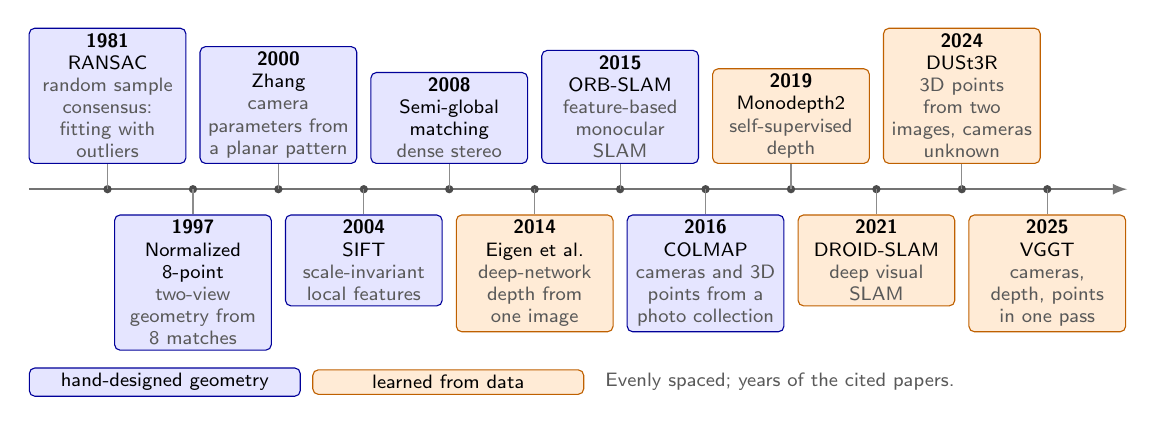
\begin{tikzpicture}[font=\sffamily\scriptsize, >=latex,
      geo/.style={draw=blue!60!black, fill=blue!10, rounded corners=2pt, align=center, text width=1.85cm, inner sep=2pt, execute at begin node=\hyphenpenalty10000},
      lrn/.style={draw=orange!75!black, fill=orange!16, rounded corners=2pt, align=center, text width=1.85cm, inner sep=2pt, execute at begin node=\hyphenpenalty10000}]
    \draw[->, thick, black!55] (0,0) -- (13.95,0);
    \foreach \x in {1.000,2.085,3.170,4.255,5.340,6.425,7.510,8.595,9.680,10.765,11.850,12.935} {\fill[black!70] (\x,0) circle (1.5pt);}
    \foreach \x in {1.000,3.170,5.340,7.510,9.680,11.850} {\draw[black!45] (\x,0) -- (\x,0.32);}
    \foreach \x in {2.085,4.255,6.425,8.595,10.765,12.935} {\draw[black!45] (\x,0) -- (\x,-0.32);}
    \node[geo, anchor=south] at (1.000,0.32) {\textbf{1981}\\ RANSAC\\ {\color{black!65}random sample consensus: fitting with outliers}};
    \node[geo, anchor=north] at (2.085,-0.32) {\textbf{1997}\\ Normalized 8-point\\ {\color{black!65}two-view geometry from 8 matches}};
    \node[geo, anchor=south] at (3.170,0.32) {\textbf{2000}\\ Zhang\\ {\color{black!65}camera parameters from a planar pattern}};
    \node[geo, anchor=north] at (4.255,-0.32) {\textbf{2004}\\ SIFT\\ {\color{black!65}scale-invariant local features}};
    \node[geo, anchor=south] at (5.340,0.32) {\textbf{2008}\\ Semi-global matching\\ {\color{black!65}dense stereo}};
    \node[lrn, anchor=north] at (6.425,-0.32) {\textbf{2014}\\ Eigen et al.\\ {\color{black!65}deep-network depth from one image}};
    \node[geo, anchor=south] at (7.510,0.32) {\textbf{2015}\\ ORB-SLAM\\ {\color{black!65}feature-based monocular SLAM}};
    \node[geo, anchor=north] at (8.595,-0.32) {\textbf{2016}\\ COLMAP\\ {\color{black!65}cameras and 3D points from a photo collection}};
    \node[lrn, anchor=south] at (9.680,0.32) {\textbf{2019}\\ Monodepth2\\ {\color{black!65}self-supervised depth}};
    \node[lrn, anchor=north] at (10.765,-0.32) {\textbf{2021}\\ DROID-SLAM\\ {\color{black!65}deep visual SLAM}};
    \node[lrn, anchor=south] at (11.850,0.32) {\textbf{2024}\\ DUSt3R\\ {\color{black!65}3D points from two images, cameras unknown}};
    \node[lrn, anchor=north] at (12.935,-0.32) {\textbf{2025}\\ VGGT\\ {\color{black!65}cameras, depth, points in one pass}};
    \node[geo, text width=3.3cm, anchor=west] at (0.0,-2.45) {hand-designed geometry};
    \node[lrn, text width=3.3cm, anchor=west] at (3.6,-2.45) {learned from data};
    \node[anchor=west, text=black!65] at (7.2,-2.45) {Evenly spaced; years of the cited papers.};
  \end{tikzpicture}}\\[0.9em]
  \begin{itemize}\footnotesize\itemsep0.3em
    \item The lecture follows this arc: the geometry first, then the learned components that replace parts of it.
  \end{itemize}
\end{frame}
